% This is a sample document using the University of Minnesota, Morris, Computer Science
% Senior Seminar modification of the ACM sig-alternate style. Much of this content is taken
% directly from the ACM sample document illustrating the use of the sig-alternate class. Certain
% parts that we never use have been removed to simplify the example, and a few additional
% components have been added.

% See https://github.com/UMM-CSci/Senior_seminar_templates for more info and to make
% suggestions and corrections.

\documentclass{sig-alternate}
\usepackage{booktabs}
\usepackage[table,xcdraw]{xcolor}
\usepackage{tabularx}
\usepackage{graphicx}
\usepackage{color}
\usepackage[colorinlistoftodos]{todonotes}
\usepackage{float}
\usepackage{wrapfig}

%%%%% Uncomment the following line and comment out the previous one
%%%%% to remove all comments
%%%%% NOTE: comments still occupy a line even if invisible;
%%%%% Don't write them as a separate paragraph
%\newcommand{\mycomment}[1]{}

\begin{document}

% --- Author Metadata here ---
%%% REMEMBER TO CHANGE THE SEMESTER AND YEAR AS NEEDED
\conferenceinfo{UMM CSci Senior Seminar Conference, December 2015}{Morris, MN}

\title{Usages of Memristors}

\numberofauthors{1}

\author{
% The command \alignauthor (no curly braces needed) should
% precede each author name, affiliation/snail-mail address and
% e-mail address. Additionally, tag each line of
% affiliation/address with \affaddr, and tag the
% e-mail address with \email.
\alignauthor
Bailey Denzer\\
	\affaddr{Division of Science and Mathematics}\\
	\affaddr{University of Minnesota, Morris}\\
	\affaddr{Morris, Minnesota, USA 56267}\\
	\email{denz0045@morris.umn.edu}
}

\maketitle
\begin{abstract}

Recently, advances in traditional computer memory technologies  have begun to decelerate as \textit{CMOS} based computing is reaching physical barriers to scaling.  This has resulted in less than spectacular improvements to performance, energy efficiency, and density.  Some researchers and companies are starting to see alternative computing architectures as viable replacements to provide continued incremental improvements to computing performance.  One such technology is the memristor developed by a research team headed by R. Stanley Williams in 2008.  These memristors are being developed in order to implement the crossbar array that has the potential to replace standard transistor based CPU architectures and many different memory formats as the memristor has the potential to be a \textit{universal memory} (a data storage device that is suitable for all types of memory storage).  It meets the requirements of a universal memory as it theoretically has read/write times faster than DRAM, densities greater than DRAM, non-volatility, long life span, and it is also suitable for performing logic.

\end{abstract}

\keywords{memristor, crossbar array, computation-in-memory, 1T1R, non-volatile, memristive}


\section{Introduction}
\label{sec:introduction}
Various aspects of modern computing technologies have begun to reach their limits.  Sustaining trends in processing speed, data storage, and energy efficiency in CMOS based computing is becoming more and more difficult as memories like DRAM and Flash begin to reach scaling limits.  Increases in CPU and memory sizes have also begun to exasperate communication bottlenecks in current computing architectures as well.  These issues have spurred research and development into alternate memory types.  The one covered in this paper is the memristor, developed in 2008 by a research team headed by R Stanley Williams \cite{MemFound}.  This memory has the potential alleviate the aforementioned issues as it has properties that make it a possible universal memory, in that it is suitable for use in both main memory and data storage due to its impressive state change times and ability to retain its state for years without power.  On top of this it has the potential to implement a computing architecture that can avoid time and energy inefficient communication bottlenecks.
%Recently, advances in traditional computer memory technologies  have begun to decelerate as \textit{CMOS}(complementary metal-oxide-semiconductor) based computing is reaching physical barriers to scaling.  This has resulted in less than spectacular improvements to performance, energy efficiency, and density.  Some researchers and companies are starting to see alternative computing architectures as viable alternatives to continue the incremental improvements to computing performance.  One such technology that has recently gained interest is the memristor developed by a Hewlett Packard research team headed by R. Stanley Williams in 2008.  These memristors are being developed in order to implement the crossbar array, which has the potential to replace traditional transistor based CPU architectures and many different memory formats as the memristor has the potential to be a \textit{universal memory} (a data storage device that is suitable for all types of memory storage).  It meets the requirements of a universal memory as it theoretically has read/write times faster than DRAM, densities greater than DRAM, non-volatility, long life span, and it is also suitable for performing logic.


Section \ref{sec:background} of this paper will first give background information on the memristor which will go over its properties as well as attempt to cover the history of the memristor.  If you plan on reading more research the history section will be more important that it would appear as it helps to clarify some confusions on what the memristor is and isn't.  A short introduction to the crossbar array will also be provided in the background.  In section \ref{lowHangers} the memristor will be compared to other memories to show how it holds up as a memory.  Then section \ref{sec:cim} one of the applications of the memristor that makes use of the crossbar array will be covered along with some results of simulations using the architecture compared to conventional computing.  To deal with a certain issue facing crossbar arrays a simple memristor cell will be shown in section \ref{sec1t1r} along with read and write time/energy models of this cell.
\section{Background Information}
\label{sec:background}

\begin{figure}
  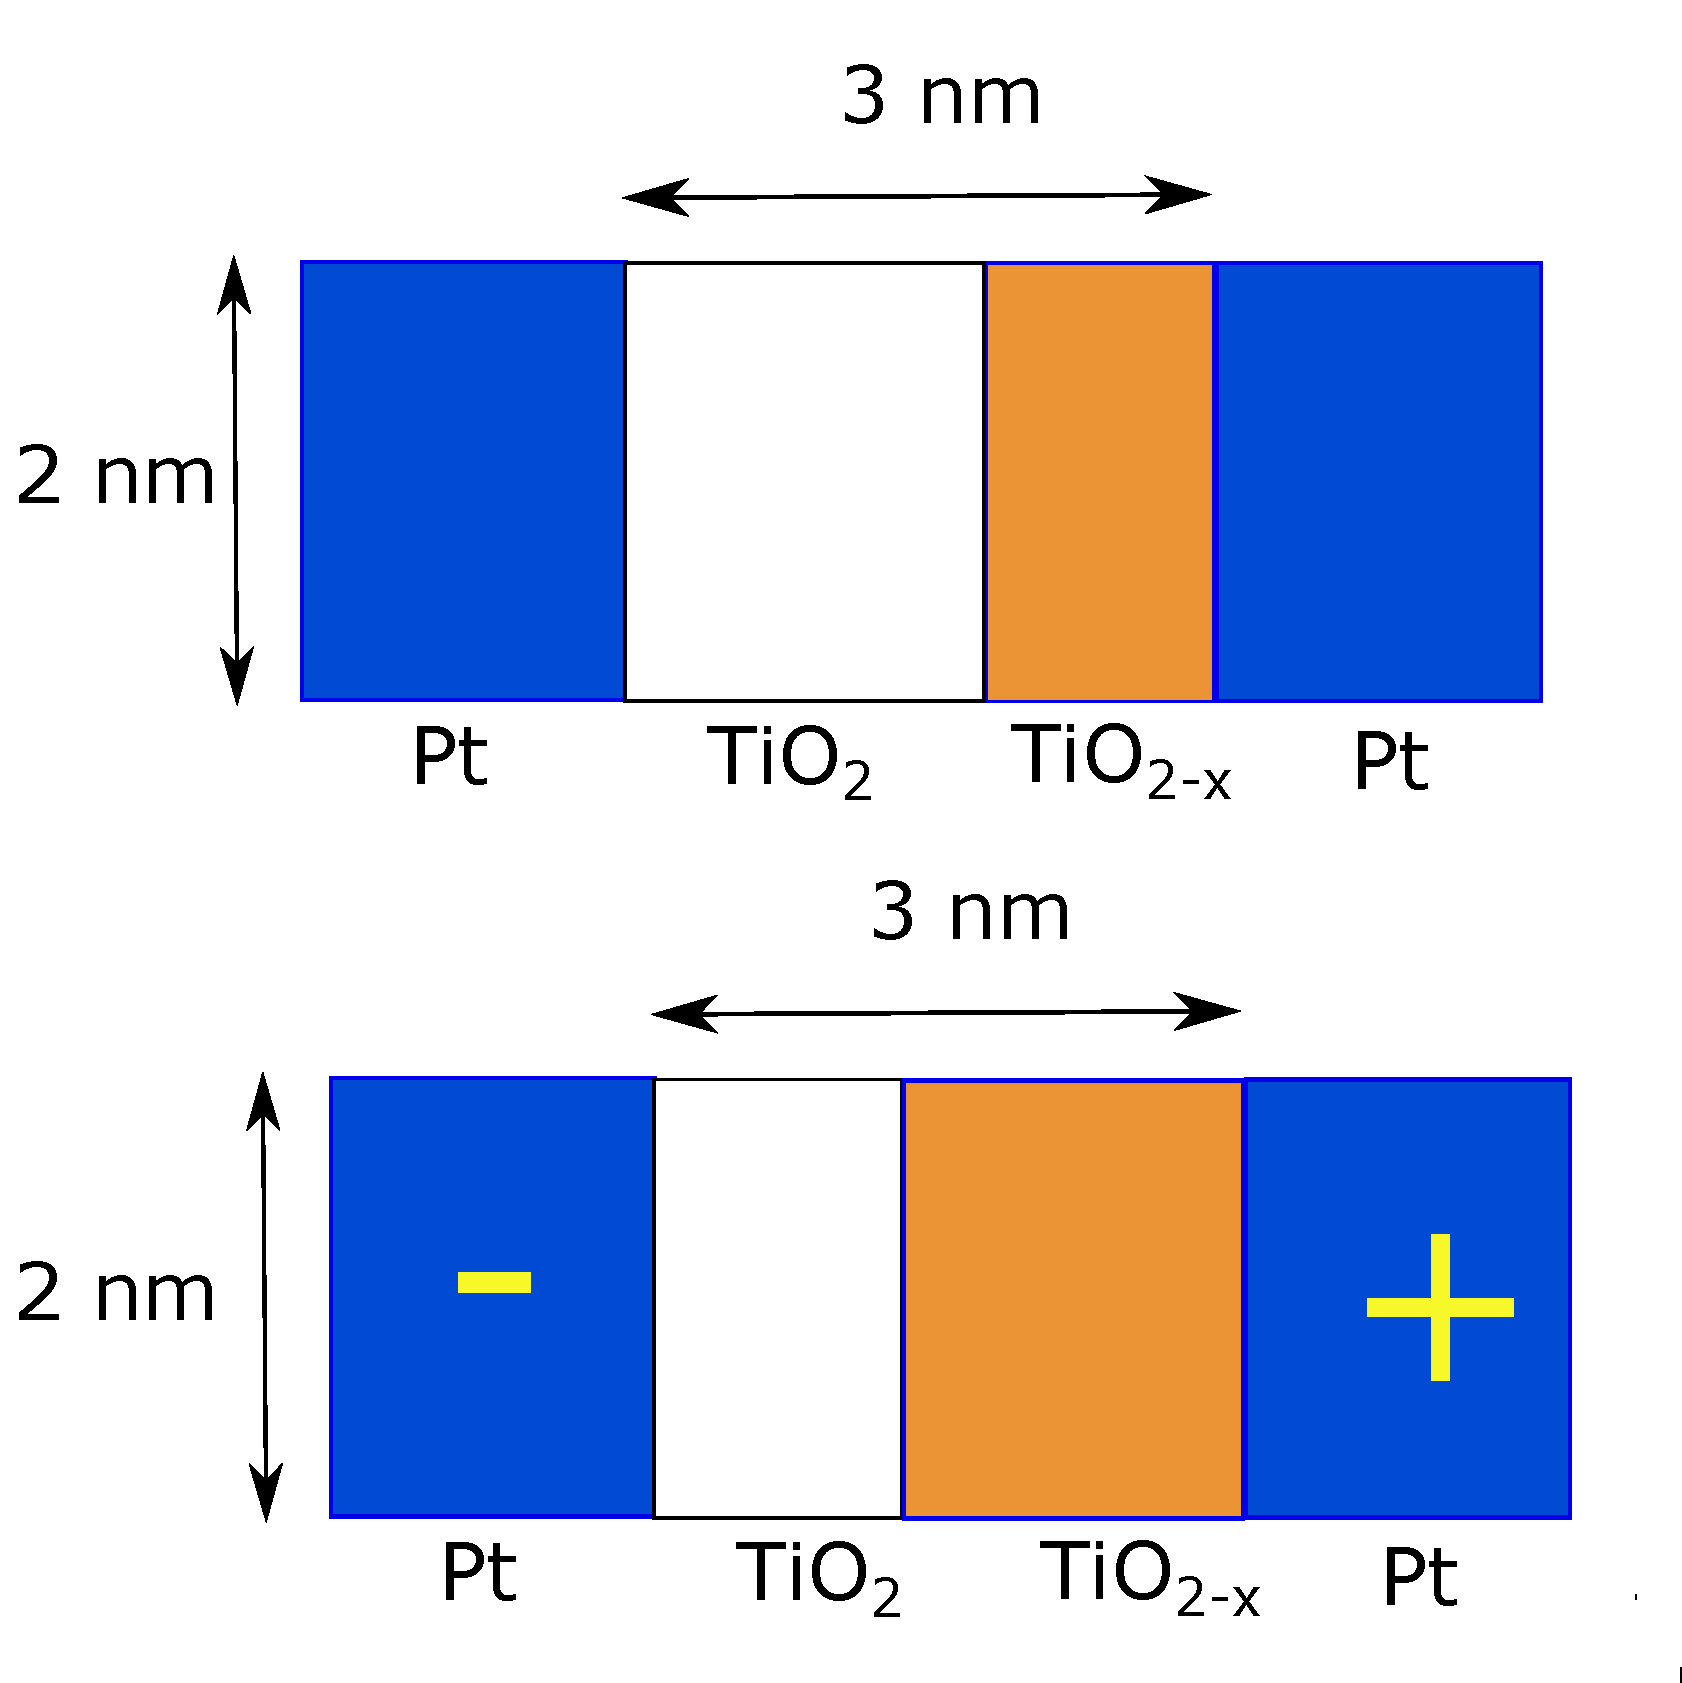
\includegraphics[width=\linewidth]{memristor.pdf}
  \caption{Simple depiction of a memristor.}
  \label{fig:memristor}
\end{figure}

\subsection{The Memristor}
\label{sec:memback}
%\label{sec:typeChangesSpecialChars}
The \textit{memristor} is a \textit{non-volatile} memory which retains information without power supply a state of resistance depending on the history of applied current.  The original memristor as depicted in Figure \ref{fig:memristor} was constructed by placing a layer of highly resistive Titanium Dioxide, $TiO_2$, and a conductive layer of $TiO_{2}$ which has had some amount of oxygen atoms removed that is represented as $TiO_{2-x}$.  These two layers are placed between two electrodes.  These electrodes would most likely be made of platinum and would be part of the crossbar array which will be covered later.  The state of the memristor is altered by passing a current through it.  This is different from more conventional memories like the volatile DRAM which stores information within a capacitor.  A capacitor with no charge would be read as a 0 and a capacitor that is fully charged would be a one.

	A more in-depth explanation of how the memristor works is as follows.  When a positive voltage is passed through the electrode on the $TiO_{2-x}$ side of the memristor it will cause vacancies to be pushed down into the $TiO_2$.  This results in the $TiO_{2-x}$ increasing in thickness while the $TiO_2$ shortens.  This increase in width of the conductive region and decrease in width of the resistive region.  It also significantly reduces the overall resistance as resistance of a material is determined by both its resistive properties and overall length.  The overall width of a memristor can constructed to be only a few nano meters or less, so it doesn't take much of a change in size of the resistive layer to have a large impact on the resistance.  This results in the memristor having a $R_{\textrm{On}}/R_\textrm{Off}$ ratio > 1000, where $R_{\textrm{Off}}$ and $R_{\textrm{On}}$ are the resistances of the memristor that correspond to 0 or 1, respectively.  This also happens fairly quickly, giving memristors switching times of nano seconds.  In order to read the memristor without disturbing its state, it is simple enough to use alternating current since alternating the current will result in no movement of the oxygen vacancies.

The memristor was originally hypothesized as the fourth missing circuit element by Chua in 1971, with the others being the resistor, capacitor, and inductor \cite{Chua}.  The theoretical memristor specifies a linkage between magnetic flux and charge.  It was not until recently in 2008 that claims of the physical realization of the memristor were made by R. Stanley Williams's research team at Hewlett Packard \cite{MemFound}.  There has been debate over whether the 2008 memristor really is the theoretical memristor.

The 2008 ``memristor" was not the first device created to exhibit memristive properties, however these devices were never claimed to be memristors.  In fact, the memristive properties of $TiO_{2}$ were known as far back as 1966, but the research was not cited by William's et al. in 2008 \cite{1968SSEle..11..535A} \cite{MemFound}.  Leon Chua replied to these criticisms in 2011 by stating that all memristive memories can be classified as memristors \cite{chua2}.   In 2015 Vongher claimed that the current ``memristor" is more than likely another implementation of existing memristive memory types, as the conceptual memristor is not possible without magnetic induction \cite{MemNotFound}.  

The HP memristor appears to be another implementation of oxidation based RRAM (resistive RAM), which uses compounds with similar properties (capable of oxygen exchanges that result in resistance changes) to the memristor to store information as resistance.  In fact, many research papers use the terms memristor and RRAM interchangeably and the HP memristor appears to specifically be redox based RRAM.  This should not affect the results of the research though, as it would appear that the physical properties of the ``memristor" are true to the explanation given above, and that the criticism is that the ``memristor" is not equivalent to the original theoretical memristor.  For simplicity and to avoid confusion I will continue to refer to the HP device as a memristor as that is what the research I am covering calls it.

\subsection{Crossbar Array}
\label{sec:cross}

When reading research on memristors it is rare to not find mention of the crossbar array.  The crossbar array is simply a collection of switches arranged in a matrix pattern. It was originally invented by HP in 2001.  From then on HP researchers were searching for a switching material with a high enough Off/On ratio to work with it.  Implementing a nano-scale crossbar array was the motivation behind the development of the memristor by R. Stanley Williams's team \cite{MemFound}.  The interest in the crossbar array is due in part to its impressive scaling capabilities (down to ~5 nm) and its simplicity allows it to be cheaply manufactured \cite{Hamdioui:2015:MBC:2755753.2757210}.  More information will be provided on the crossbar array in the CIM section. (Still thinking about where everything should go, might move all crossbar array things up here).


\begin{table}
  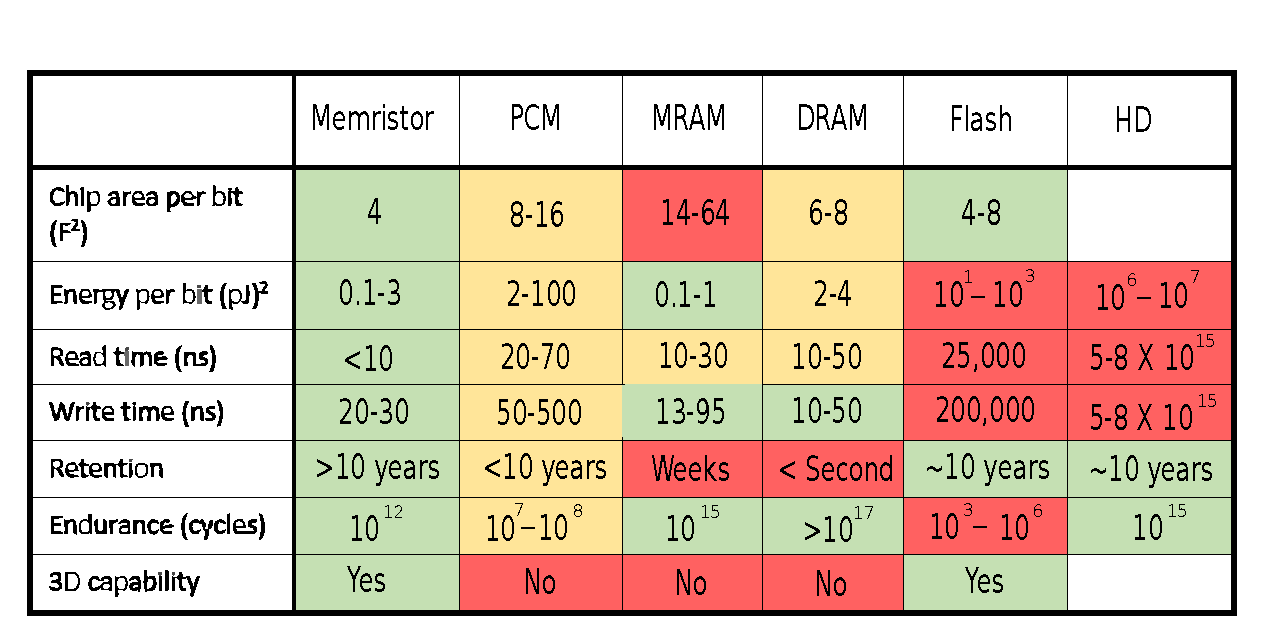
\includegraphics[width=\linewidth]{Comparison-of-Data-Storage-2updated8.pdf}
  \caption{\cite{HPmemStuff} Comparison of different memories.  From left to right: PCM is phase change memory, STT-RAM is MRAM (magnetic RAM), DRAM (dynamic RAM) is currently used for main memory, NAND or flash memory used in SSD's, and HD.  At the moment everything other than DRAM, NAND, and HD are under development}
  \label{table:DATA}
\end{table}
\label{sec:inlineEquations}


%\section{Memristor Based Architectures}

\section{Memristors as Memory}
\label{lowHangers}
One of the most obvious uses of memristors is as a memory.  Table \ref{table:DATA} provides a chart of some of the advantages memristors have over other memory storage types \cite{HPmemStuff}.  The source is from an article by HP, but comparing the results to similar RRAM tables these results seem to be accurate.  They have significant advantages in density, read/write time, data retention, cycles (endurance), and energy consumption.  Crossbar arrays allow them to be densely stacked into a three dimensional block with the potential to store petabytes of memory within a cubic centimeter.  Not shown in the chart, memristors have also drawn particular interest as they can potentially be cheaply manufactured using techniques for manufacturing traditional CMOS technology.  When looking at the table it would also appear that DRAM is only slightly less energy efficient than memristors but this is not true.  What is shown is the power to access a bit of DRAM once, but it does not account for the fact that DRAM must continually be refreshed, causing it to consume large amount of power relative to the other memories in the table.  

The last three columns are memories that most are familiar with.  When referring to RAM for computers that is usually referring to DRAM, the main memory that the CPU accesses.  DRAM has the highest endurance, roughly five orders of magnitude higher than memristors, so it may be possible that memristors would have some trouble being used as main memory due to endurance issues.  Both Flash and HD are used for mass storage as their read and write times are too long and they are not bit accessible like RAM as memory is accessed in chunks rather than on a per bit basis.  

The other two memories after memristors are still in development however they have yet to hit the market in any meaningful way despite being in development for much longer than memristors.  They both have some similarities to memristors as they are both non-volatile RAM's and are being developed as possible replacements to current memory types.  STT-RAM or spin transfer torque RAM is the newest implementation of magnetoresistive RAM.  It has the lowest power consumption on the table as well as the second highest endurance and respectable read/write times, but it suffers from having a large feature size.  Similar to the memristor, phase change memory stores a state as resistance, and it was even argued by Leon Chua that it should be classified as a type of memristor \cite{chua2}.  Its method of changing its resistance is significantly different though and it is temperature sensistve as temperature is used to change its state.  This memory appears to have some drawbacks compared to memristors and even DRAM.  Both PCM and STT-RAM will not likely be manufactureable using techniques used in manufacturing CMOS like the memristor \cite{pcm} \cite{stt}.  

The memristor also has plenty of room for improvement.  The original memristor was made using $TiO_2$, however there have been memristors made using other materials with excellent properties.  For example a more recent implementation useing tantalum oxide has been shown to have switching times from 105 to 120 pico seconds, or one-hundredth of the write times shown in Table \ref{table:DATA} \cite{0957-4484-22-48-485203}.

\section{CIM - Computation in Memory}
\label{sec:cim}

\subsection{Von Neumann Bottleneck}

Modern computing designs are based off Von Neumann architecture.  In this architecture the CPU and main memory are two physically separate things that communicate through buses.  A diagram of how this communication works is shown in Figure \ref{fig:crossbar} \cite{vonnewt}.  The transfer of information through these buses results in the Von Neumann Bottleneck where the data transfer rate is significantly less than the data that needs to be transferred.  To make things worse the bus can only access either the CPU or main memory, not both at the same time.  This results in the data transfer rate being lower than speed at which the CPU can work by forcing it to wait for information.  This problem has been getting worse as both main memory size and CPU speeds have increased much faster than the data transfer rates.  The transfer of data is also highly energy intensive.  It is estimated that communication of data takes up 70 to 90\%\ of energy consumption, leaving only 10 to 30\%\ of energy consumption for performing computations              \cite{Hamdioui:2015:MBC:2755753.2757210}.  For example, executing a multiply instruction in 45nm technology uses about 70 pJ, where as the actual operation only uses 4 pJ.

There are several methods for mitigating the Von Neumann bottleneck but the problem persists.  Some of these methods include using SRAM caches or providing an on chip CPU stack.  It is interesting to note that these methods are essentially attempts at bringing the memory closer to the CPU.  SRAM caches have their own limitations though as they have poor density, expensive to manufacture, and are experiencing increasing energy leakage is they are increasingly scaled down.
%Memristors are not restricted to applications as memory storage.  CIM (computation in memory) is being proposed by \cite{Hamdioui:2015:MBC:2755753.2757210} as a replacement for traditional Von Neumann (VN) architecture for use in data-intensive applications.  Figure \ref{fig:Computer_system_bus} gives a diagram of how information is exchanged in Von Neumann architecture.  With traditional architecture processing and data storage are performed in physically separate locations.  This results in the need for large amounts of data transfer between the two.  Von Neumann architecture has some draw backs that the CIM architecture can address.  
%For data intensive computations, having large amounts of data being transferred back and forth between the processor and memory can result in the processors being unable to reach their maximum performance as the processor needs to wait for information transfer, and energy inefficiency as the data transfer can be costly.  It is estimated that communication of data takes up 70 to 90\%\ of energy consumption in VN architecture, with the rest being used for actual computation \cite{Hamdioui:2015:MBC:2755753.2757210}. This is a result of the processor-memory bottleneck, often called the Von Neumann bottleneck.  Within the crossbar array that CIM utilizes, the memristors can be dynamically chosen to be used for either gates or data storage.  This allows large portions of the crossbar array to be set up so that data necessary to a computation can be physically stored next to the memristors that have been converted into gates.  This removes the need to be constantly accessing things like SRAM caches which have high energy consumption, poor density (due to the fact that it takes between 4 to 10 transistors to represent a bit in SRAM), and information bottle-necking.  The motivation behind realizing a CIM architecture is to eliminate the communication bottleneck, support massive parallelism, and reduce energy inefficiency.  


\begin{figure}
  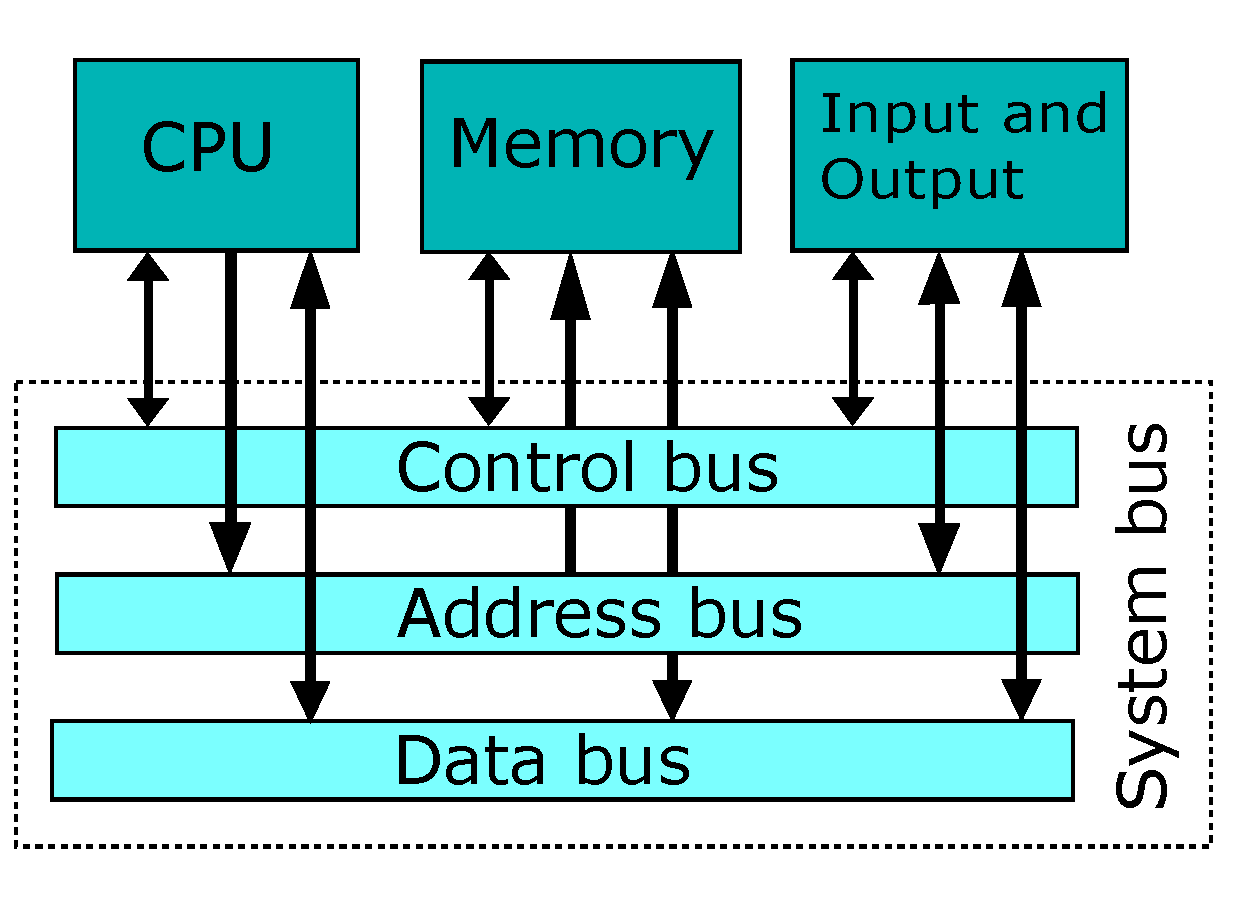
\includegraphics[width=\linewidth]{Computer_system_bus.pdf}
  \caption{Communication in Von Neumann architecture}
  \label{fig:crossbar}
\end{figure}


\subsection{Basic Design}
A solution to the Von Neumann bottleneck is to have the CPU and main memory merged as proposed by Hamdioui et al \cite{Hamdioui:2015:MBC:2755753.2757210}.  In CIM the computation and data storage are integrated in a crossbar array.  Memristors in a crossbar array can be used for data storage and logic which allows computations and memory to be integrated into the same chip.  This removes the need for data transfer through buses that have poor data transfer rates.  This also removes the need to be constantly accessing things like SRAM caches which have high energy consumption, poor density (due to the fact that it takes between 4 to 10 transistors to represent a bit in SRAM), and information bottle-necking.Since the crossbar array has such high densities and the memristors themselves have little to no power leakage and good read/write switching time, there would be enough room for these to be combined without needing to increase the size of the processor to match the total storage and processing power of a conventional architecture.
A more succinct overview of the advantages of CIM is as follows:
\begin{itemize}
\item Tightly integrated (scalable to ~5nm) computation-in-memory crossbar
architecture supporting massive parallelism.

\item Little to no power leakage.  Current VN architectures are beginning to run into scaling problems due to power leakages from constantly accessing SRAM caches.

\item Significant performance improvement at lower energy and area.
\end{itemize} 

The memristor based crossbar construction also uses materials and designs that CMOS manufacturing techniques can be applicable to.  Outside of the crossbar array, the control and communication can be made using standard CMOS based technology, but it would require a significant redesign to be compatible with a CIM architecture.  Because of this, the research paper from Hamdioui et al. is proposing CIM as a concept and does not appear to have a fully designed architecture at hand.  Computations of this architecture are simulated based an assumptions of how the architecture would behave.

%A crossbar array is constructed out of electrodes in a tic-tac-toe pattern with (for example) the horizontal bars being above and the horizontal bars being below.  There is a small gap between them though, allowing memristors to be placed between them at the junctions.

%\begin{figure}
%  \begin{center}
%  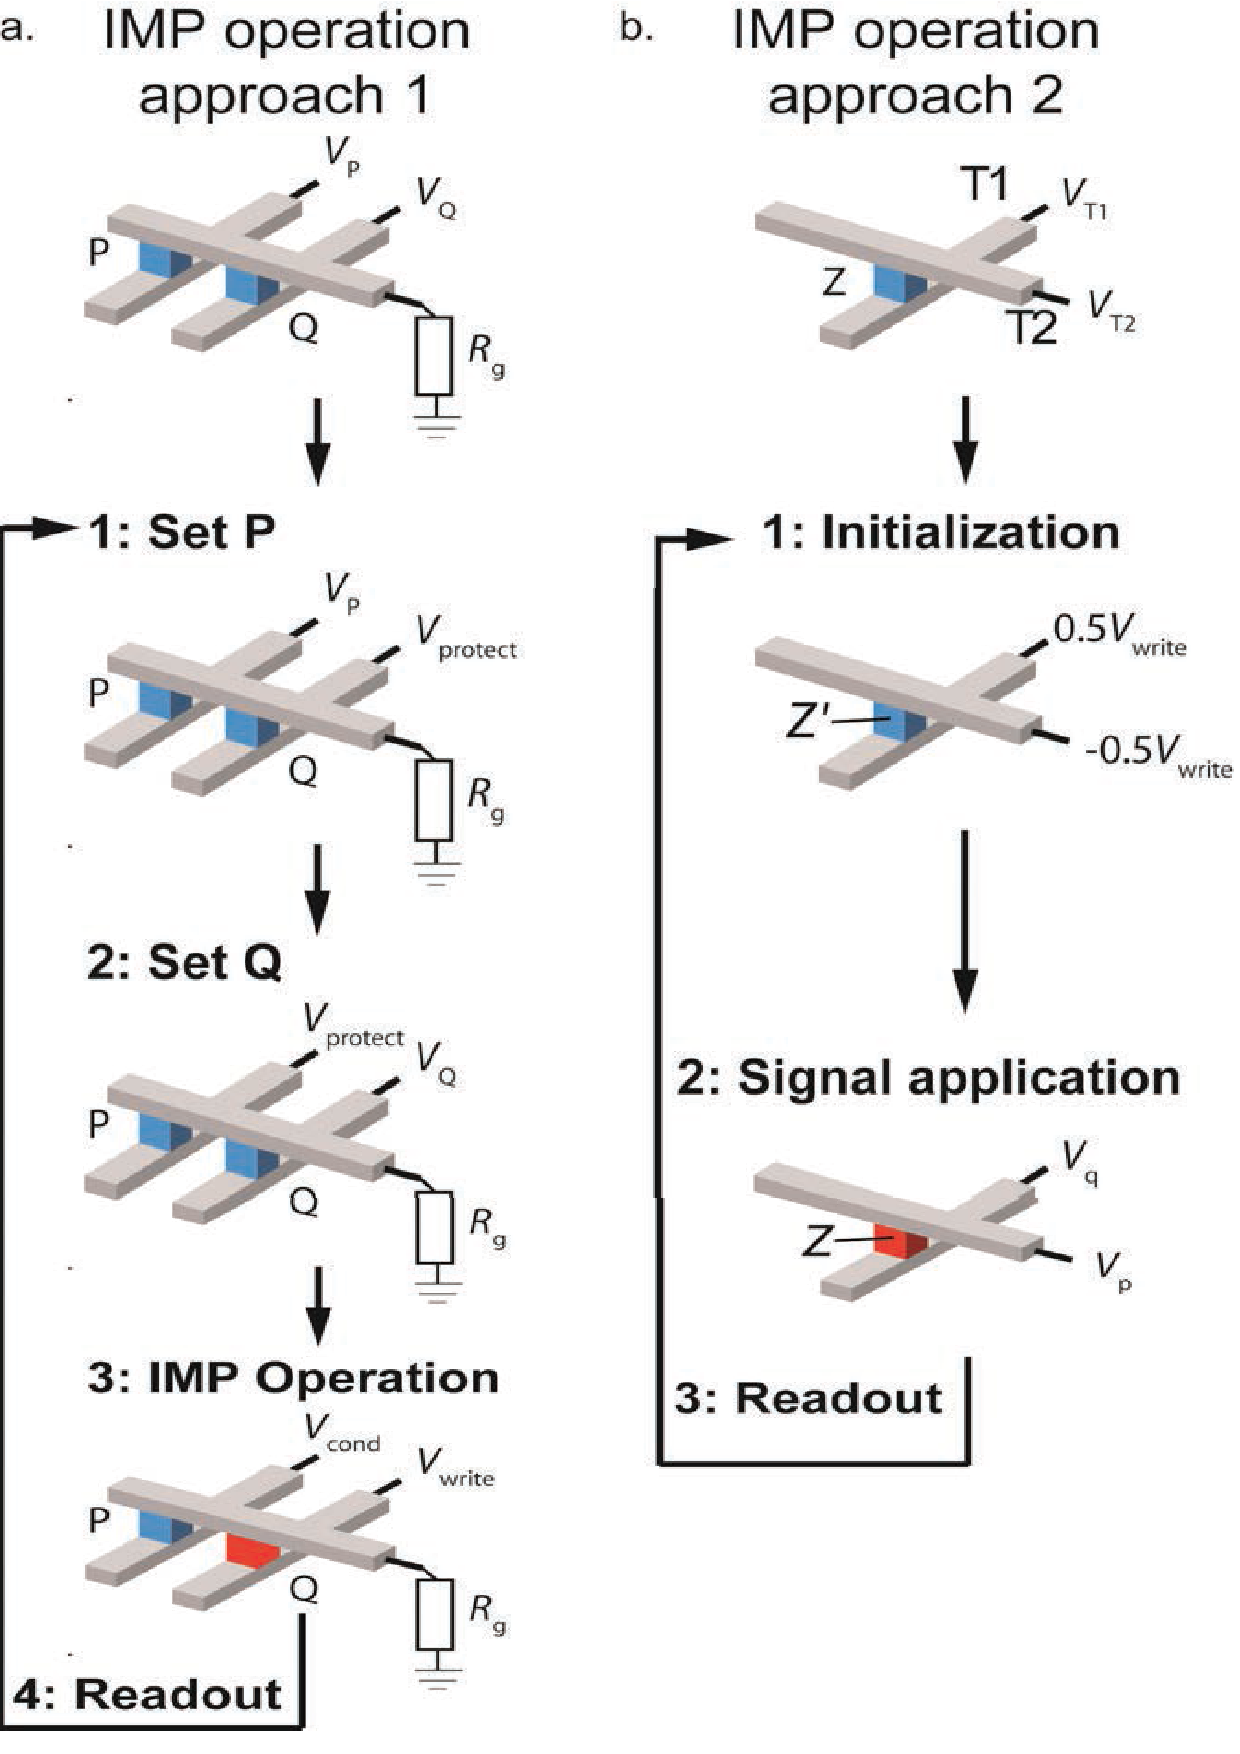
\includegraphics[scale=.3]{imp.pdf}
%  \caption{IMP}
%  \end{center}
%  \label{fig:inmemcrossbar}
%\end{figure}


%A short explanation of how IMP works is as follows.  Input signals as voltages $ Vp = \pm \frac{1}{2} V_{write} $ and $ Vq = \pm \frac{1}{2} V_{write} $ are applied to the terminals T1 and T2 in Figure \ref{fig:inmemcrossbar} (I'am unsure why this reference is not correct), where $V_{write}$ is a specified voltage to be applied during a write procedure.  This operation will store the resistance state of Z.  In an example where we want to set Z to a value corresponding to bit 1:

%1. Init device Z to '1' $(VT1 = + \frac{1}{2} V_{write}, VT2 = -\frac{1}{2} V_{write}$)

%2. $Z' = p$ IMP $q (VT1 = Vq, VT2 = Vp)$

%3. Read $Z'$

\subsection{Results on Large Data-sets}
\label{sec:theoremLikeConstructs}

\begin{table}
  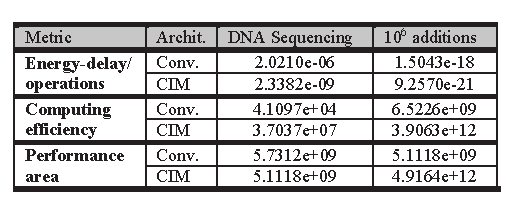
\includegraphics[width=\linewidth]{results.pdf}
  \caption{Results of simulated data-sets.  Unfortunately the source only used these as comparisons, and did not provide any actual units. }
  \label{tab:results}
\end{table}

Table \ref{tab:results} displays the simulated results between conventional and CIM architecture from \cite{Hamdioui:2015:MBC:2755753.2757210}.  The DNA sequencing results were computed by performing a common solution for comparing two DNA sequences in which a sorted index of reference DNA is created in order to identify the locations of matches or mismatches in another sequence.  In the particular case set up by Hamdioui et al. they are comparing 200 GB of DNA data to 3GB of healthy reference. The other example is for $10^6$ parallel addition operations.  The first row of the table represents the the energy-delay product per operations, the second row the computation efficiency defined as the number of operations per required energy, and the third row is the number of operations per area. These simulations were based off of a fairly large table of assumptions provided by Hamdioui et al. \cite{Hamdioui:2015:MBC:2755753.2757210}.
%Some of the assumptions appear to be questionable though, as their assumption on the read time for a memristor is 200 ps which they cited from ITRS which is a fairly reputable source.  However this read time does not match up with what other sources are reporting which is closer to 2 ns, roughly 10 time what is being assumed here.  Because of this, it is likely that the results are more realistically one or two orders of magnitude in difference, rather than 3.


\begin{figure}
  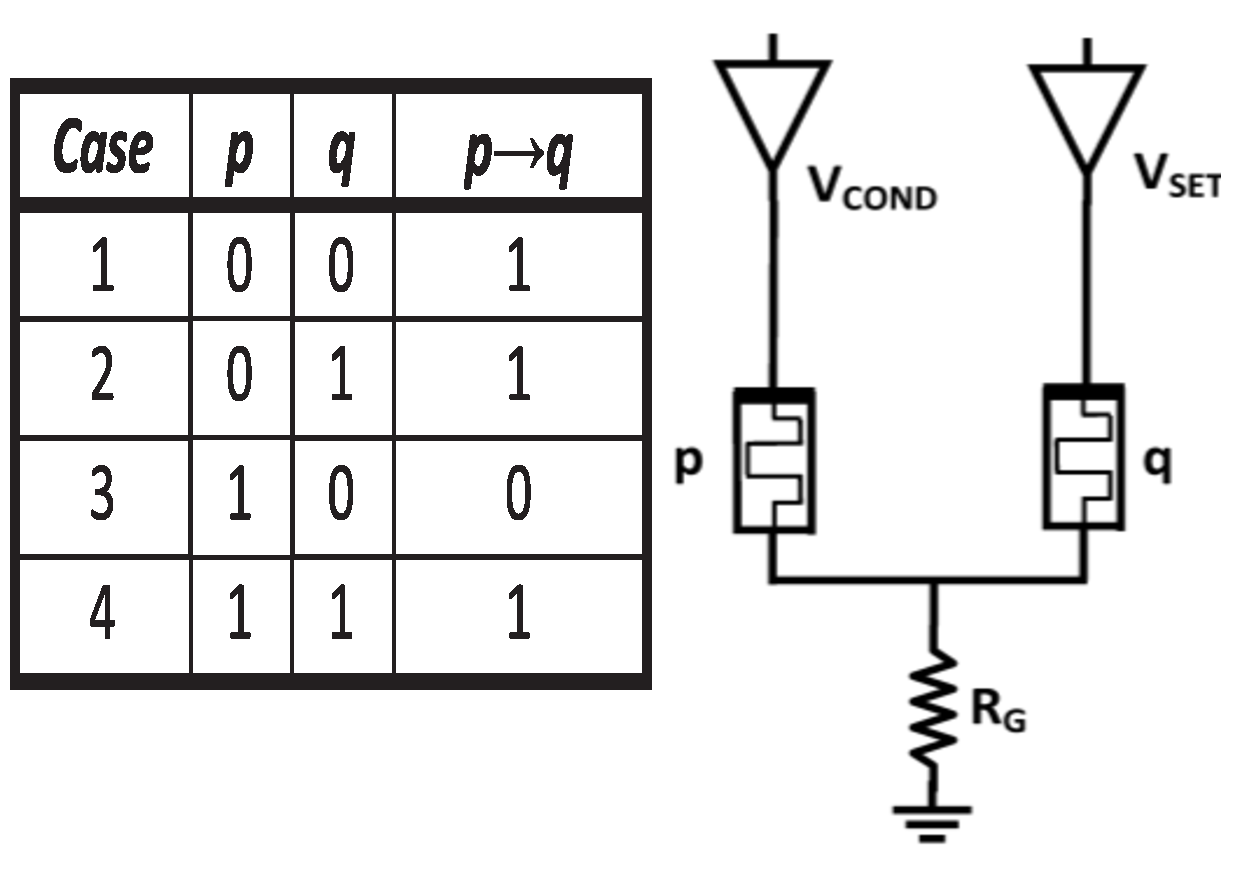
\includegraphics[scale=.28]{imply.pdf}
  \caption{The imply function.  The initial values of p and q are the input bits, with q being the output bit after applying the voltages $V_{\textrm{set}}$ and $V_{\textrm{cond}}$ }
  \label{fig:imply}
\end{figure}

\subsection{How Memristors Function as Logic Switches}



%\begin{figure}
%  \begin{center}
 % 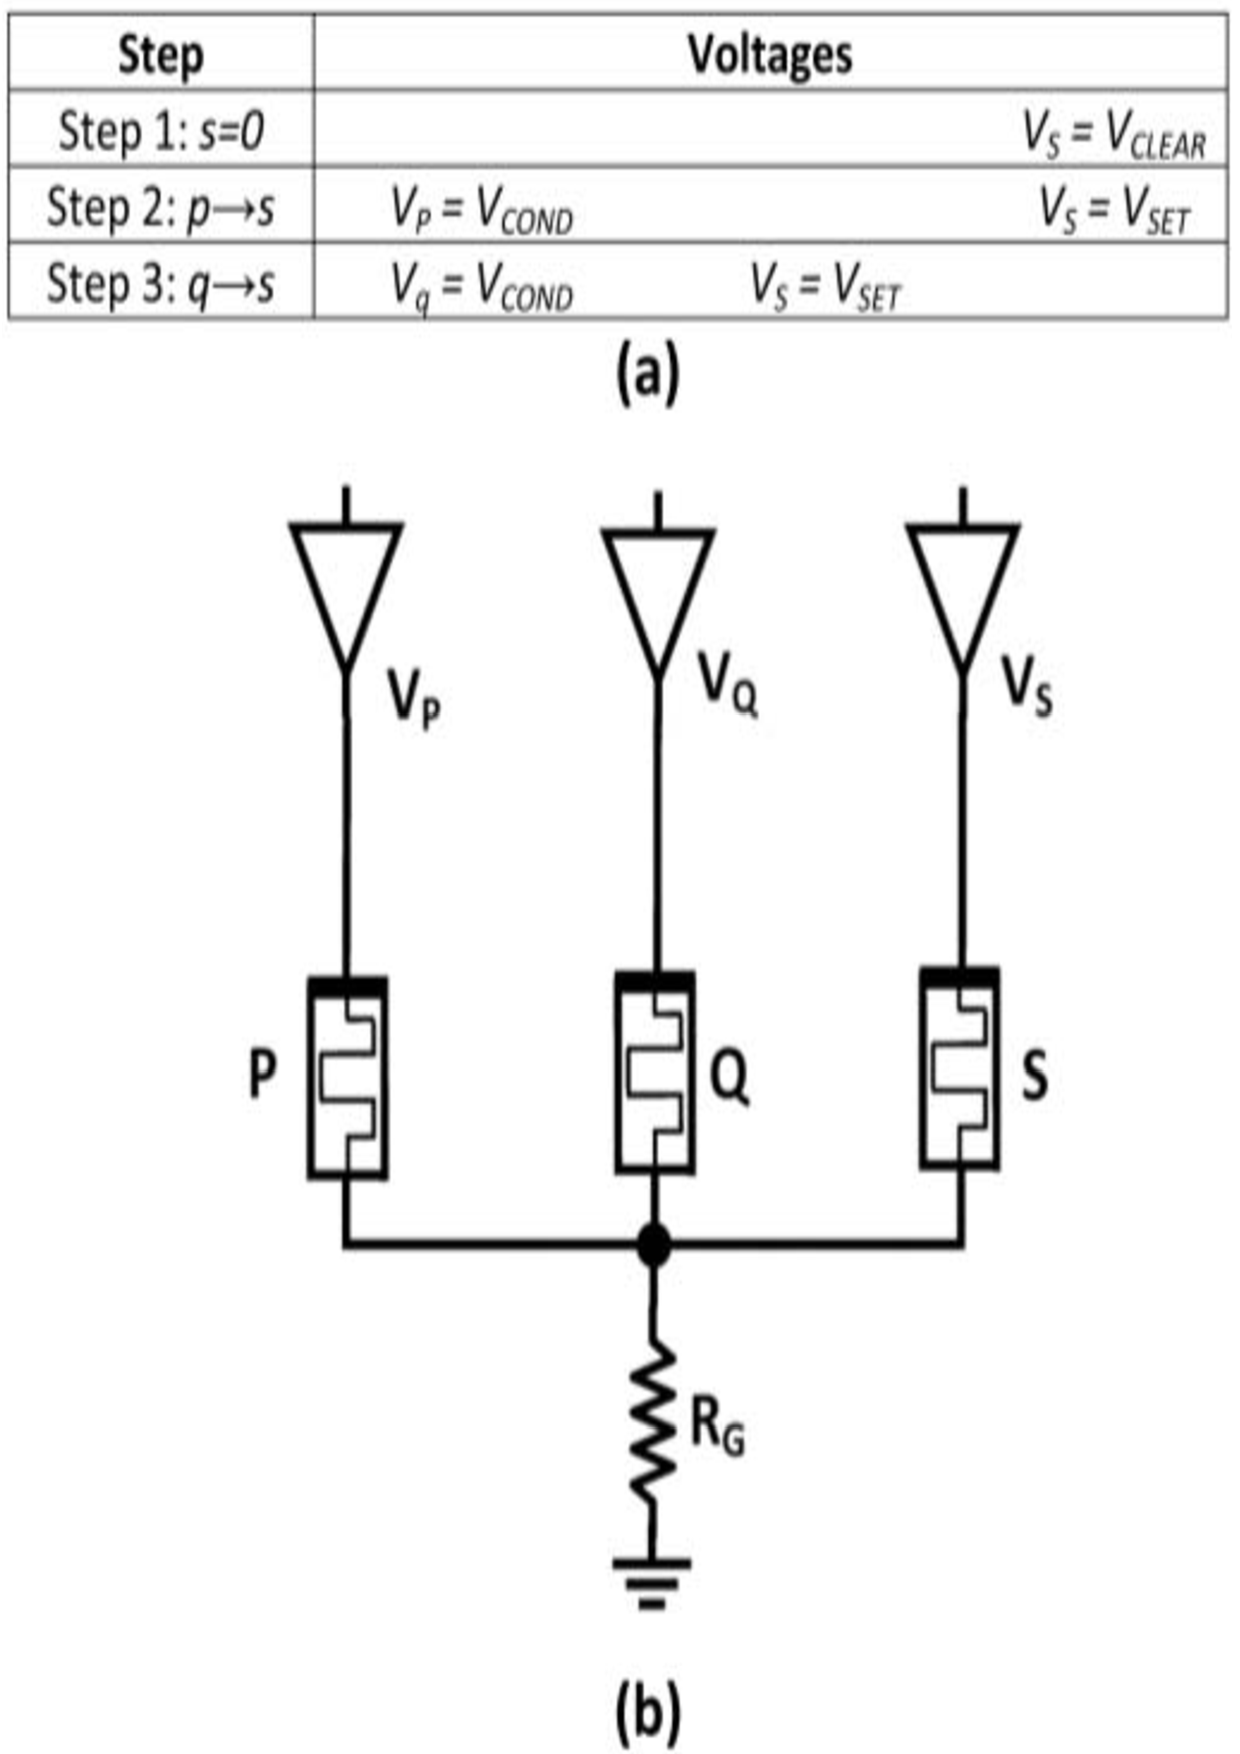
\includegraphics[scale=.28]{andImp.pdf}
%  \caption{A nand gate using IMP logic \cite{kvatinsky2014memristorbased}}
%  \end{center}
%  \label{fig:andImp}
%\end{figure}
%An example of an imply based nand gate along with the steps that occur in its execution is shown in Figure \ref{fig:andImp}.  
An interesting thing about memristors is that they do not implement the same logic that conventional transistor based gates would.  In order to perform logic in a memristor crossbar array architecture, material implication logic (IMP) is used.  A truth table of the imply function along with an imply logic gate is given in Figure \ref{fig:imply} \cite{kvatinsky2014memristorbased}.  Just like nand gates imply gates are capable of implementing any boolean function, allowing for crossbar arrays of memristors to perform any logic functions.  In either of the gates the memristors are connected to a resistor $R_{G}$ where the resistance of $R_{G}$ is between $R_{\textrm{Off}}$ and $R_{\textrm{On}}$. What exactly happens during the imply gate with memristors P and Q with initial states p and q is as follows:

\begin{itemize}
\item Apply voltage $V_{\textrm{cond}}$ to P and $V_{\textrm{set}}$ to Q 
where (|$V_{\textrm{cond}}| < |V_{\textrm{set}}$|)
\item If p = 1 (low resistance), the voltage on the shared terminal is approximately $V_{\textrm{cond}}$ and the voltage on Q is $V_{\textrm{set}} - V_{\textrm{cond}}$, which is small enough that the state of Q is unchanged.
\item If $p = q = 0$ (high resistance), then the resistance on Q is approximately  $V_{\textrm{set}}$, and Q is switched to 1.
\item If p = 0 and q = 1, the state of Q is also unchanged.
\end{itemize}

%\subsection{1T1R}
%\label{sec:caveatForExperts}

%Another useful application for memristors is RRAM cells which could potentially replace current forms of memory such as SRAM, DRAM, and Flash memory.  [2] proposes to construct RRAM (resistive random access memory) using a standard CMOS (complementary metal-oxide semiconductor) transistor paired with a memristor.  

%(Still figuring out how to condense down the information from the research paper on this topic)

\begin{figure}
  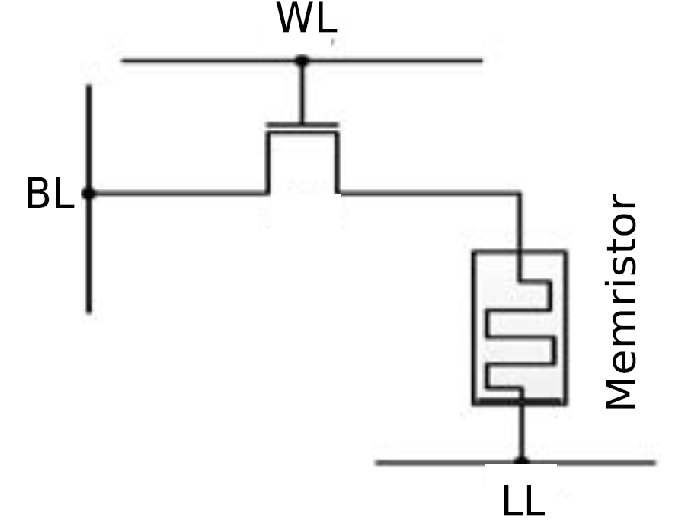
\includegraphics[scale=.29]{1t1real.png}
  \caption{1T1R cell: BL = Bitline, WL = Wordline}
  \label{fig:crossSwitch}
\end{figure}

\begin{figure}
  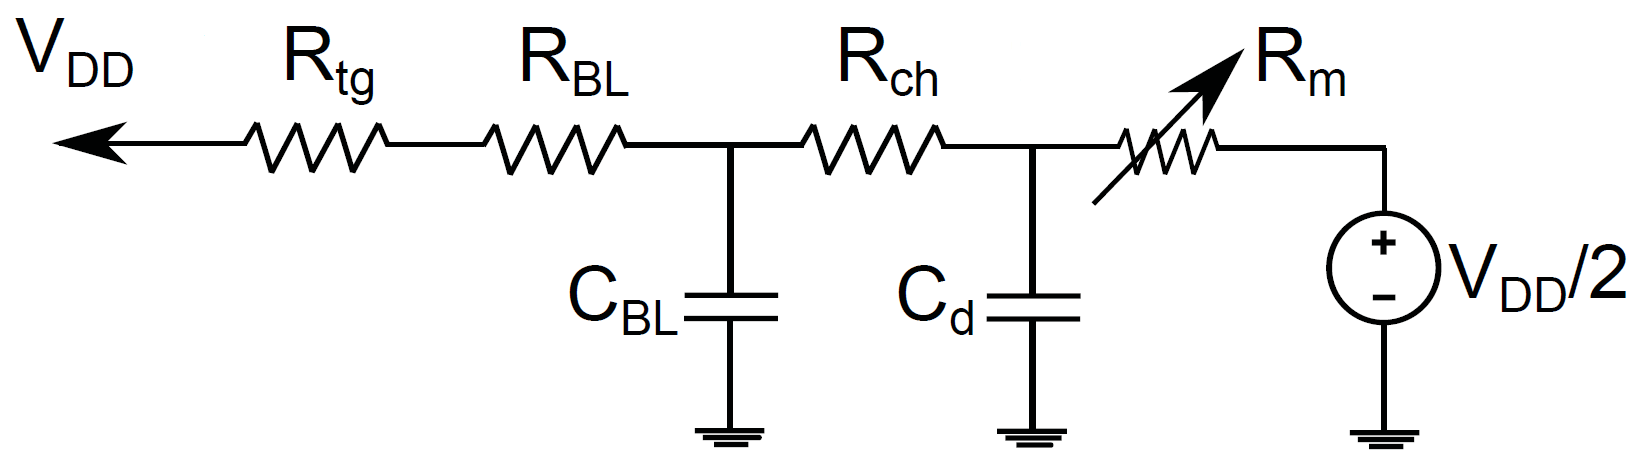
\includegraphics[scale=.2]{1t1rwrite.png}
  \caption{Circuit of a 1T1R cell during a write.  $V_{BL}$ is set to $V_{DD}$ for writing 1, and 0 for writing 0.}
  \label{fig:1t1rite}
\end{figure}

\section{1T1R}
\label{sec1t1r}
One of the main problems with the crossbar array is the sneak path problem.  Since electricity always looks for a path with the least resistance, there is little preventing the previously described crossbar array from having what is called a sneak path.  This results when an alternative path is made when reading/writing where instead of going through the desired memristor, the current may instead travel through different memristors.  This is far from an unsolved problem as there are multiple ways of dealing with this, but one method in particular is the 1T1R cell as proposed by Zangeneh et al. \cite{Zangeneh:2012:PEM:2206781.2206786}.  It stands for one transistor, one resistor (in this case the resistor is a memristor) and has some parallels with DRAM cells, as they are made up of one transistor, one capacitor.  A 1T1R equivalent cell during a write operation is shown in figure \ref{fig:crossSwitch}.  

Out of the methods for dealing with the sneak-path problem this one appears to be the simplest and has the highest access times.  The memristor used in this is the standard $TiO_2$ based one.
Like DRAM, the proposed 1T1R architecture has a wordline to select a row of cells and a bitline to select columns.  During a write a voltage $V_{DD}$ is applied to the wordline, and a positive or negative voltage is applied across the memristor for writing 1 or 0 logic.  This is done by either charging the bitline to $V_{DD}$ (for logic 1) or discharging it to 0 $V$ (for logic 0), and applying a voltage $\frac {V_{DD}}{2}$ at node LL.

This implementation would likely not be the best choice to use in the aformentioned CIM architecture.  While it would still allow for data storage and computation within the same region, it would be less than ideal to be replacing transistors in a processor with a transistor/memristor hybrid.  

\subsection{Read/Write Properties of 1T1R}
This subsection will provide the four main equations for the read and write models, regarding the time to read/write and the energy to read/write.  Comparing the results of the models to the results to Table \ref{fig:DATA}, they seem to agree with each other.  Figure \ref{fig:1t1rite} provides a circuit diagram during a write procedure.  

\subsubsection{Write Time Model}
\begin{figure}
  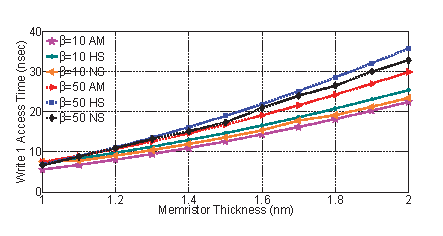
\includegraphics[scale=1.2]{writetime.pdf}
  \caption{Analytical model vs HSPICE simulations for write 1
access time as a function of memristor thickness for different
$\beta$(On/Off ratio). AM = Analytical model ignoring bitline capacitance,
HS = Hspice simulations and NS = Numerical solution
accounting for bitline capacitance.}
  \label{fig:writeTime}
\end{figure}
The equation to model the time necessary to write to a memristor is:
\begin{equation*}
T_{w} = \frac{L^2 (1 + \beta)}{2 \mu _{v} V_{A}}
\end{equation*}

In this equation the T in $T_{w}$ stands for time and the subscript w stands for write.  $L$ is the thickness of the memristor, $\beta$ is the ratio of $R_{\textrm{Off}}$ and $R_{On}$, $V_{A}$ is the magnitude of the applied voltage, and $\mu _{v}$ is a constant for the mobility of the oxygen vacancy.  According to this equation then, if the thickness of the memristor or the difference in resistance between an off state and on state increase, then the time to write will increase.  If the applied voltage is increased the time to write will decrease.  Using this model a read time of approx. 7 ns was found with $\beta = 10$ and $L = 1 nm$ when writing a 1, but when writing a 0 with the same parameters it can be as low as 4 ns. A graph of the model is provided in Figure \ref{fig:writeTime} \cite{Zangeneh:2012:PEM:2206781.2206786}.

\todo[inline]{There's some ugly gaps between the last two figures in this section.  They've been that way for quite a while and changing their sizes does nothing.  Not sure of how to fix it yet.}
\subsubsection{Read Time Model}

\begin{figure}
  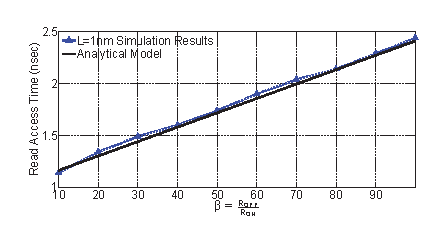
\includegraphics[scale=1.2]{readtime.pdf}
  \caption{Read time model: Analytical model versus HSPICE simulation results
for read access time of the 1T1R cell as a function of $\beta$ for
different memristor thicknesses L.}
  \label{fig:readTime}
\end{figure}
The equation to model the time required to read is:
\begin{equation*}
T_{R} = 0.69(R_{ch} + R_{BL} + R_{\textrm{Off}})C_{BL}
\end{equation*}
$R_{ch}$ is the resistance of the access transistor, $R_{BL}$ is the resistance of the bitline resistor, and $C_{BL}$ is the bitline capacitance. Figure \ref{fig:readTime} provides an illustration with $R_{ON}$ = 100 $\Omega$, $R_{tg}$ = 582 $\Omega$ , and  $C_{BL}$ = 200 fF \cite{Zangeneh:2012:PEM:2206781.2206786}.  

\subsubsection{Write Energy Model} 

\begin{figure}
  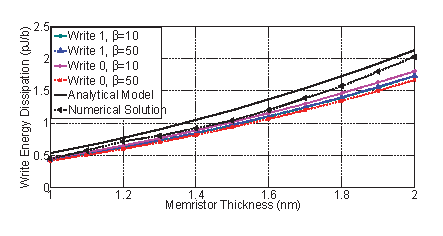
\includegraphics[scale=1.2]{writeenergy.pdf}
  \caption{ Write Energy Model: Analytical model ignoring the bitline capacitance and Numerical solution considering bitline capacitance.}
  \label{fig:writeEnergy}
\end{figure}

The model for energy consumption during a write procedure is:
\begin{equation*}
E_{w} = \frac{V_{DD}I_{1}}{2(\zeta)}
\end{equation*}
$I_{1}$ is $\int_{.1}^{.9} \frac{1}{1-x^4} dx$, the integral of the inverse of the window function which models the nonlinear rate of state change of a memristor and $\zeta = \frac{\mu _{v}R_{ON}}{L^2}$.  Figure \ref{writeEnergy} graphs the model as a function of memristor thickness with $(R_{tg} = 582 \Omega$, $R_{ON} = 100 \Omega ,$ and $C_{BL} = 200fF)$ \cite{Zangeneh:2012:PEM:2206781.2206786}.

\subsubsection{Read Energy Model} 
\begin{figure}
  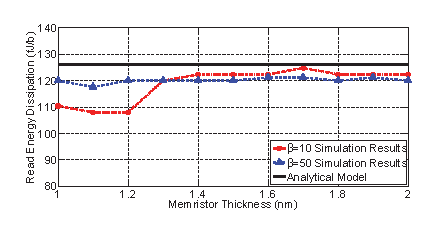
\includegraphics[scale=1.2]{readenergy.pdf}
  \caption{Comparison between the proposed model and HSPICE simulations of read energy.}
  \label{fig:readEnergy}
\end{figure}
The model for energy consumption during a read procedure is:
\begin{equation*}
E_{R} = 0.63C_{BL}V^2_{DD}
\end{equation*}

Figure \ref{fig:readEnergy} provides a graph of the model, with $R_{On} = 100 \Omega $, $C_{BL} = 200fF$, which shows that the energy to read is independent of memristor thickness \cite{Zangeneh:2012:PEM:2206781.2206786}.

\section{Other Applications}
Aside from memory and logical computations, memristors have many other potential uses.  One usage in particular that comes up often is its use in neural networks.  There is much research applying memristors to simulate synapses in cognitive computing since memristance is somewhat analogous to how synapses behave.  The more a synapse is used the stronger its connection becomes, similar to how a memristor can become more conductive as a current is applied to it.  This makes memristors a prime candidate for storing information not to be interpreted as a binary number but as a range of values that could represent a synapse \cite{5713299}.
\section{Conclusions}
\label{sec:conclusions}

As covered in the paper, the memristor appears to be a promising new device for high density, high speed, and energy efficient computing.  This paper should have also made the history of the memristor a little more understandable as it is somewhat complicated.  It has been shown to be suitable for new computing architectures that do not suffer from a communications bottleneck.  It also has the potential to replace many of the mediums for data storage such as NAND and DRAM as it appears to be a prime candidate as a universal memory.  There is still likely much to do before memristors start replacing transistors in processors, but the potential is there.

\section*{Acknowledgments}
\label{sec:acknowledgments}
Thanks to Elena Machkasova, Nic McPhee and Will Martin for reviewing the paper.


% The following two commands are all you need in the
% initial runs of your .tex file to
% produce the bibliography for the citations in your paper.
\bibliographystyle{abbrv}
% sample_paper.bib is the name of the BibTex file containing the
% bibliography entries. Note that you *don't* include the .bib ending here.
\bibliography{sample_paper}  
% You must have a proper ".bib" file
%  and remember to run:
% latex bibtex latex latex
% to resolve all references

\end{document}
